\documentclass{article}
\usepackage{tikzpeople}
\usepackage{tikz}
\usetikzlibrary{shapes, shapes.misc}
\usetikzlibrary{arrows, arrows.meta, decorations.markings}
\usetikzlibrary{patterns}

%\usetikzlibrary{calc,backgrounds}
%\usepackage[active,tightpage]{preview}
% taken from manual
\makeatletter
\pgfdeclareshape{document}{
\inheritsavedanchors[from=rectangle] % this is nearly a rectangle
\inheritanchorborder[from=rectangle]
\inheritanchor[from=rectangle]{center}
\inheritanchor[from=rectangle]{north}
\inheritanchor[from=rectangle]{south}
\inheritanchor[from=rectangle]{west}
\inheritanchor[from=rectangle]{east}
% ... and possibly more
\backgroundpath{% this is new
% store lower right in xa/ya and upper right in xb/yb
\southwest \pgf@xa=\pgf@x \pgf@ya=\pgf@y
\northeast \pgf@xb=\pgf@x \pgf@yb=\pgf@y
% compute corner of ‘‘flipped page’’
\pgf@xc=\pgf@xb \advance\pgf@xc by-10pt % this should be a parameter
\pgf@yc=\pgf@yb \advance\pgf@yc by-10pt
% construct main path
\pgfpathmoveto{\pgfpoint{\pgf@xa}{\pgf@ya}}
\pgfpathlineto{\pgfpoint{\pgf@xa}{\pgf@yb}}
\pgfpathlineto{\pgfpoint{\pgf@xc}{\pgf@yb}}
\pgfpathlineto{\pgfpoint{\pgf@xb}{\pgf@yc}}
\pgfpathlineto{\pgfpoint{\pgf@xb}{\pgf@ya}}
\pgfpathclose
% add little corner
\pgfpathmoveto{\pgfpoint{\pgf@xc}{\pgf@yb}}
\pgfpathlineto{\pgfpoint{\pgf@xc}{\pgf@yc}}
\pgfpathlineto{\pgfpoint{\pgf@xb}{\pgf@yc}}
\pgfpathlineto{\pgfpoint{\pgf@xc}{\pgf@yc}}
}
}
\makeatother

\begin{document}
\begin{center}

\resizebox{\textwidth}{!}{%
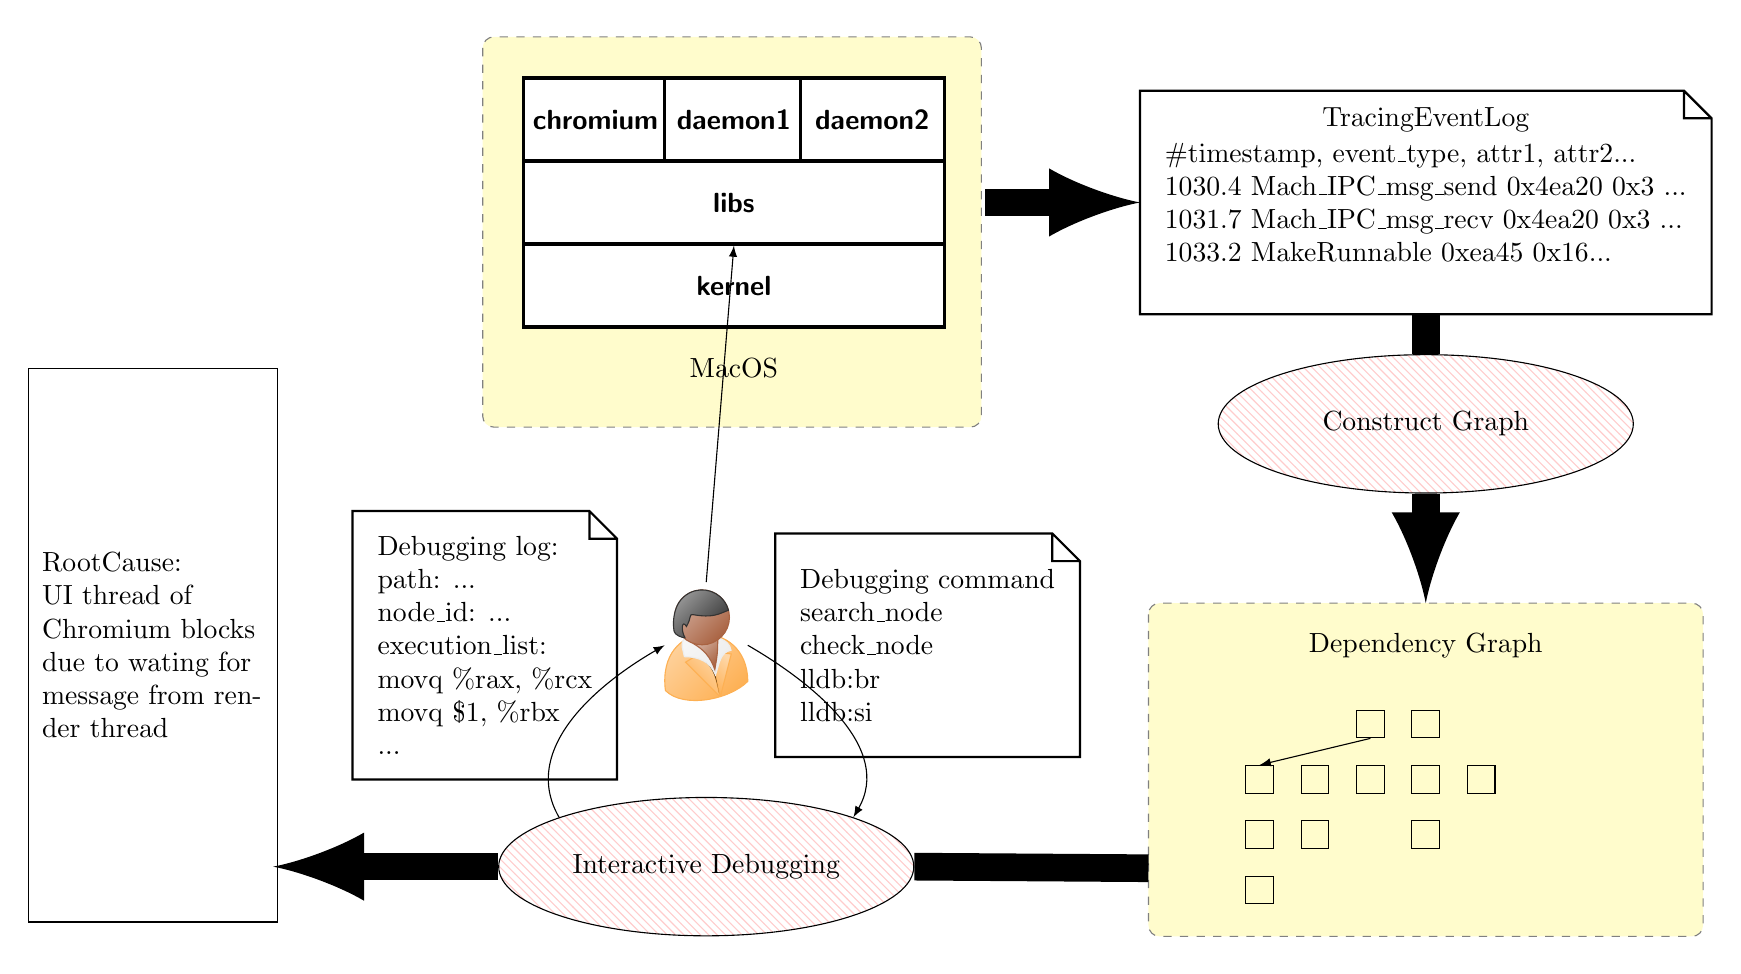
\begin{tikzpicture}[>=latex]
% We need layers to draw the block diagram
\pgfdeclarelayer{background}
\pgfdeclarelayer{foreground}
\pgfsetlayers{background,main,foreground}

\tikzstyle{apps} = [draw, very thick, minimum height=3em, minimum width=5em, fill=white, rectangle, font={\sffamily\bfseries}]
\tikzstyle{systemComp} = [draw, very thick, minimum height=3em, minimum width=15.2em, fill=white, rectangle, font={\sffamily\bfseries}]
\tikzstyle{actionLabel} = [draw, pattern=north west lines, pattern color = red!20, ellipse, minimum width = 15em, minimum height= 5em]%shape aspect=3, minimum size=30, diamond]

\tikzstyle{doc} = [draw, thick, align=left, color=black, shape=document, minimum width=20em, minimum height=8em, shape=document, inner sep=2ex]
\tikzstyle{commanddoc} = [draw, thick, align=left, color=black, shape=document, minimum width=5em, minimum height=8em, shape=document, inner sep=2ex]
\tikzstyle{debuglogdoc} = [draw, thick, align=left, color=black, shape=document, minimum width=8em, minimum height=8em, shape=document, inner sep=2ex]
\tikzstyle{mininode} = [draw, rectangle, minimum height=1em, minimum width=1em]

\tikzstyle{prearrow} = [-, thick, line width=1em] %double distance = 1.2em, shorten >=-0.2em]
\tikzstyle{vecarrow} = [->, thick, line width=1em] %double distance = 1.2em, shorten >=-0.2em]
%\tikzstyle{vecarrow} = [thick, decoration={markings, mark=at position
   %1 with {\arrow[xshift=1.2em, scale=0.6] {triangle 90}}},
   %1 with {\arrow[xshift=1.5em]{Straight Barb[length=2pt 0.7]}}},
   %double distance=1.2em,
   %postaction= {decorate}]

%draw MacOS components
\node [apps, name=software1] at (0, 0) {chromium};
\node [apps, name=software2, right of=software1, node distance=5em] {daemon1};
\node [apps, name=software3, right of=software2, minimum width=5.2em, node distance=5em] {daemon2};
\node [systemComp, name=libs, below of=software2, node distance=3em] {libs};
\node [systemComp, name=kernel, below of=libs, node distance=3em] {kernel};
\node (MacOS) [below of = kernel, minimum width=15em, node distance = 3em] {MacOS};

% draw Tracing Event log
\node (TracingEventLog) [minimum height=3em, minimum width=20em, right of=software3, node distance=20em] {TracingEventLog};
\node [doc, below of=TracingEventLog, name=log, node distance=3em] {\#timestamp, event\_type, attr1, attr2...\\1030.4 Mach\_IPC\_msg\_send 0x4ea20 0x3 ...\\1031.7 Mach\_IPC\_msg\_recv 0x4ea20 0x3 ...\\1033.2 MakeRunnable 0xea45 0x16...};

%draw arrow from MacOS to Tracing Event log
%\draw[vecarrow, shorten >= -0.05em] (libs.east)+(0.5, 0) -- (log.west);%(TracingEventLog.west);
\draw[vecarrow] (libs.east)+(0.5, 0) -- (log.west);%(TracingEventLog.west);

%draw Arrow for Constructing Graph
\node [actionLabel, below of=log, node distance=8em, name=action1] {Construct Graph};
\draw [prearrow] (log.south) -- (action1.north);

%draw Dependency Graph
\node (DependencyGraph) [minimum height=3em, minimum width=20em, below of=action1, node distance=8em] {Dependency Graph};
\node [mininode, below of=DependencyGraph] (1c3) {};
\node [mininode, left of=1c3, node distance=2em] (1c2) {};
\node [mininode, below of=1c2, node distance=2em] (2c2) {};
\node [mininode, left of=2c2, node distance=2em] (2c1) {};
\node [mininode, left of=2c1, node distance=2em] (2c0) {};
\node [mininode, right of=2c2, node distance=2em] (2c3) {};
\node [mininode, right of=2c3, node distance=2em] (2c4) {};
\node [mininode, below of=2c0, node distance=2em] (3c0) {};
\node [mininode, right of=3c0, node distance=2em] (3c1) {};
\node [mininode, right of=3c0, node distance=6em] (3c2) {};
\node [mininode, below of=3c0, node distance=2em] (4c0) {};
\draw [->] (1c2.south) -- (2c0.north);
\node (DGendline)[minimum height=1em, minimum width=20em, below of=DependencyGraph, node distance=10em]{};

%\draw [vecarrow, shorten <=-0.2em, shorten >= 0.1em] (action1.south) -- (DependencyGraph.north);
\draw [vecarrow] (action1.south) -- (DependencyGraph.north);

%draw interactive Debugging part
\node [commanddoc, left of=DependencyGraph, node distance=18em](command){Debugging command\\search\_node\\check\_node\\lldb:br\\lldb:si};
\node[alice, minimum size=3em, left of=command, node distance=8em](user) {};
\node [debuglogdoc, left of=user, node distance=8em](debuglog){Debugging log:\\path: ...\\node\_id: ...\\execution\_list:\\  movq \%rax, \%rcx\\  movq \$1, \%rbx\\  ...};
\node [actionLabel, below of=user, node distance=8em, name=action2] {Interactive Debugging};
\draw [->] (user.east) to [out=330,in=60] (action2.north east);
\draw [->] (action2.north west) to [out=120,in=210] (user.west);
\draw [->] (user.north)+(0, 0.1) to (libs.south);
\draw [prearrow](DGendline.north west) + (0, 0.5) -- (action2.east);
%\draw [prearrow, -, shorten >= -1.8em](DGendline.north west) + (0, 0.5) -- (action2.east);
%\node (result) [draw, rectangle, align=left, minimum height=2em, minimum width=20em, below of = action2, node distance=6em] {RootCause:\\UI thread blocking in Chromium because of\\wating for message from Render thread};
%\draw [vecarrow, shorten <= -0.2em] (action2.south) -- (result.north);

\node (result) [draw, rectangle, align=left, minimum height=20em, minimum width=9em, text width=8em, left of=debuglog, node distance=12em] {RootCause:\\UI thread of Chromium blocks due to wating for message from render thread};
\node (alignresult)[left of=action2, node distance=16em]{};
%\draw [vecarrow, shorten <= -1.8em] (action2.west) -- (alignresult.east);
\draw [vecarrow] (action2.west) -- (alignresult.east);

\begin{pgfonlayer}{background}
%%draw background rectangle for macos, graph and debugging log
\path (software1.west |- software3.north)+(-0.5, 0.5) node (a) {};
\path (MacOS.south east)+(0.5, -0.5) node (b) {};
\path[fill=yellow!20,rounded corners, draw=black!50, dashed] (a) rectangle (b);
%%draw backgroud for dependancy graph
\path (DependencyGraph.west |- DependencyGraph.north) node (a) {};
\path (DGendline.south east) node (b){};
\path[fill=yellow!20,rounded corners, draw=black!50, dashed] (a) rectangle (b);
%%draw background for interactive debugging
%\path (IDbeginline.west |- IDbeginline.north) node (a) {};
%\path (IDendline.south east) node (b) {};
%\path[fill=yellow!20,rounded corners, draw=black!50, dashed] (a) rectangle (b);

\end{pgfonlayer}
\end{tikzpicture}
}
\end{center}
\end{document}
